\section{Literature Review}

The literature review section will cover a few important topics necessary to understand the research being conducted. The video game environment will be introduced, explained and provide arguments why they were chosen for this research. This will be followed by an explanation of each algorithm chosen and why they were chosen to be compared. Finally, the literature review will cover similar works conducted in the field of RL in pokémon and how they compare to the research being conducted.

\subsection{Introduction to Pokémon Red}

Pokémon Red is a role-playing game where the player controls a character navigating through the world in order to defeat the eight Gym Leaders and the Elite Four. The game is played from a top-down perspective and the player controls the actions of the main character within a grid. The player has to navigate the main character around the overworld, interact with non-player characters, and battle with wild Pokémon and other trainers. An example of how the world is percieved by the player is provided below\cite{HubZ_1998}. 

\begin{figure}[H]
    \centering
    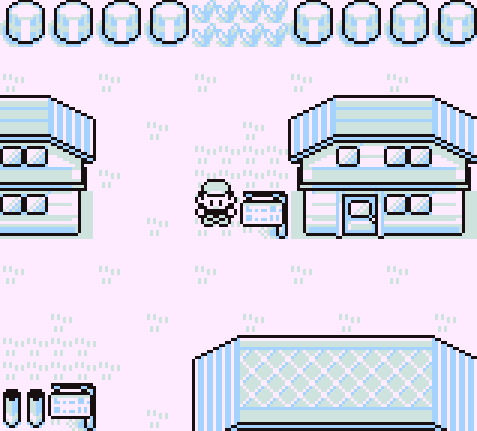
\includegraphics[width=0.5\textwidth]{figures/red_pallet_town.png}
    \caption{Example of Pokémon Red Overworld}
    \label{fig:pkmn_overworld}
\end{figure}

As seen in figure \ref{fig:pkmn_overworld}, the game's overworld map uses a tile based system, where each tile represents a different type of terrain with some being traversable and others are not. The player can see what is visible on the screen and interpret the small sprite images on each tile to understand what is happening. However, the player has these pre-conceived notions of what each tile represents and what each sprite represents, which is not present in the agent initally \cite{HubZ_1998}. 

Moreover, the game includes text boxes that provide information to the player about the game's story and what next immediate objective is. The game is aimed at younger audiences, implying that the language is simple and easy to understand. However, the agent does not have the same understanding of the language as a human would. The agent instead interprets the set of pixels on the screen representing the text and through trial and error tries to understand what to do \cite{HubZ_1998}. 

\begin{figure}[H]
    \centering
    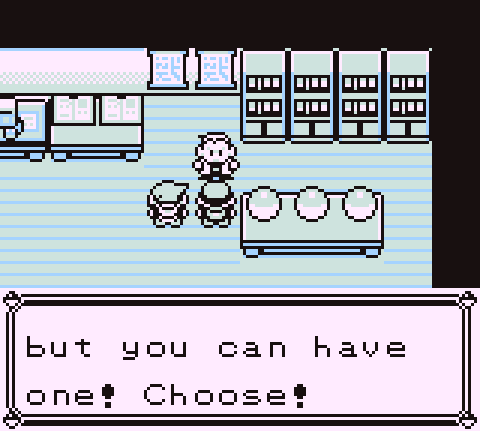
\includegraphics[width=0.5\textwidth]{figures/red_quest_example.png}
    \caption{Example of a Quest}
    \label{fig:pkmn_quest}
\end{figure}

The game's battling is turn-based, where the player selects Pokémon moves for their Pokémon to perform in battle. This turn-based battling system is very similar to rock-paper-scissors, where the player and opposing challenger has to choose a pokémon move for their pokémon to perform before knowing what the other has chosen. However, it is far more in-depth, as each pokémon has varying levels of effectiveness, strength and consequence. Every turn while in battle, the player has to make a decision on what move to perform, which is the most effective to swiftly defeat their opponent. The menu where this takes place can be seen in figure \ref{fig:pkmn_battling} \cite{HubZ_1998}.

\begin{figure}[H]
    \centering
    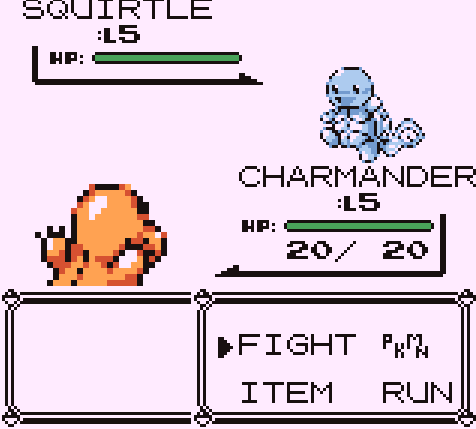
\includegraphics[width=0.5\textwidth]{figures/red_battling.png}
    \caption{Example of a Pokémon Battling}
    \label{fig:pkmn_battling}
\end{figure}

The game has a large number of items and moves that the player can use to their advantage in battle and while navigating within the overworld. Therefore, there is a large amount of potential possible decisions while playing the game making each playthrough of the game unique while keeping goals consistent during each play through\cite{HubZ_1998}.

As the player progresses through the game, they will encounter different types of Pokémon of all shapes and sizes, as well as watch their pokémon grow in strength as it levels up. Each pokémon has a set of numerical values that determine how strong, fast and resilient they are. These values increase as the pokémon grows which is how the player can determine how powerful their pokémon is. The player can also catch wild pokémon to add to their team, which can be used to battle other trainers and wild pokémon. All of these factors combined make the game a complex environment full of different small choices which will stick with the player for the rest of the game. An example of the player's starting pokémon numerical values are shown in figure \ref{fig:pkmn_stats} \cite{HubZ_1998}.

\begin{figure}[H]
    \centering
    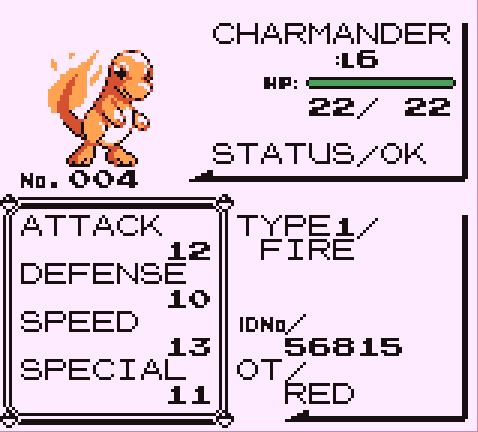
\includegraphics[width=0.5\textwidth]{figures/red_stats.png}
    \caption{Example of a Pokémon Numerical Values}
    \label{fig:pkmn_stats}
\end{figure}

As mention before, the game is a long game that takes up to 25 hours to complete, therefore it is not designed to be completed in one sitting. This can be seen by the number of different towns and cities the player has to navigate through solving puzzles and defeating gym leaders along the way. The map of the world within the game can be seen  in figure \ref{fig:pkmn_map} \cite{HubZ_1998}. 

\begin{figure}[H]
    \centering
    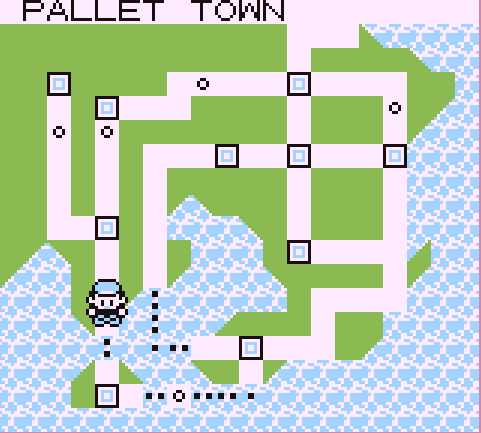
\includegraphics[width=0.5\textwidth]{figures/red_map.png}
    \caption{Pokémon World Map}
    \label{fig:pkmn_map}
\end{figure}

\subsection{Why Pokémon Red?}

One reason why the video game Pokémon Red was chosen for this research project was due to its complexity and the large number of possible actions the agent can take. Within the field of RL, video games are very common environments to train agents with, as they an effective way to train an agent to perform a task within a simulated world. However, only short arcade style games such as the Atari games have been used as a benchmark where it surpassed human performance for every listed game \cite{brockman2016openai}. The exception to this is openAI's Dota 2 agent, which was able to defeat the world champion team. However, the agent was trained for 10 months using state of the art hardware, which is far beyond the scope of this research \cite{berner2019dota}.

The atari games used to benchmark different RL algorithm performances lack long term randomness, complexity and decision making, where present actions influencing future states and future decisions \cite{brockman2016openai}. This is present within pokémon red, as it takes 25 hours to complete, where every tiny decision made at every minute has an influence on the future \cite{howlongtobeat}. An example of this would be the decision of which pokémon to catch and train or which pokémon you start your journey with. Moreover, the game is a good representation of multi-objective goals. This is because the agent cannot complete the game if it is able to navigate the map confidently but avoid battling, and on the other hand, the agent cannot complete the game if it chooses to only battle and not explore the map.

\subsection{Why choose RL?}

Within the field of machine learning, there are multiple different forms of learning that can be applied to the environment of pokémon red. However, due to the depth of the action space of the environment and the limitations of other forms of machine learning, RL is the best form of machine learning to explore how to find the optimal path to completing the game. 

The biggest drawback when using supervised or unsupervised learning is the dataset. The dataset would need someone playing the game for countless hours completing the game or reaching a checkpoint in the game before starting a new episode from that point \cite{XanderSteenbrugge2019intro}. Not only is this method increcible slow, as humans can only play and operate at a certain speed, but the dataset would also never experience actions that are unnatural for a human to perform, as the dataset is bound to the actions a human would take with the human's preconception of how to play the game. This leads onto the other issue, where the dataset of human playing the game is bound by human constaints. Humans are naturally lazy and have short attention spans, which means when providing the training data knows one way to solve a puzzle, they are unlikely to experiment other methods in solving the puzzle \cite{XanderSteenbrugge2019intro}. Therefore, the agents trained on the human provided data are bound and limited by the performance of the human and will never surpass the training data finding a more optimal path. 

RL is the solution to finding the set of actions to complete the game as it allows the agent to 'play' the game itself and explore the environment in a sped-up space to find the optimal path without the need of a human to show it how to play, while knowing what the goal is. 

\subsection{Deep Q Networks (DQN)}

DQN is a value based off-policy algorithm that learns by optimizing a value function to maximize reward in the long term. DQN was developed developed by combining RL techniques and deep neural networks at scale by enhancing the Q-Learning algorithm with deep neural networks and a technique called experience replay \cite{TFAgentsAuthors2023}.

Q-Learning is based on the Bellman equation, where the agent learns the optimal action-value function by iteratively updating the Q-values of the state-action pairs \cite{mnih2013playing}. The Q-value of a state-action pair is the expected return of taking the action in the current state, where the value of a state is the sum of the immediate reward and the discounted value of the future states \cite{bellman1958dynamic}. It is impractical to explore the Q-values of every state-action pair, as the state space of the environment is too large to computationally check \cite{mnih2013playing}. Instead, a function approximator such as a deep neural network is used to estimate unexperienced Q-values. 

Q-Learning is an off-policy algorithm, meaning that there is a seperate behavior policy for interacting with the environment. In DQN, the behavior policy is an epsilon-greedy policy. The episolon-greedy policy selects the action with the highest Q-value with a probability of $1 - epsilon$ and selects a random action with $epsilon$ probability \cite{TFAgentsAuthors2023}. The epsilon-greedy policy is used to balance the exploration and exploitation of the agent within the environment, as exploration and exploitation is what determines how often the agent should enter unexperienced observations and therefore fill out the Q-table. Balancing out exploration and exploitation is important as exploitation is dependent on the current known best set of action and exploration is required to enter new states and discover states yielding higher reward \cite{TFAgentsAuthors2023}.

Value based algorithms, such as DQN, learn the environment by optimizing a value function, where it expects a high amount of value to be returned in the long term \cite{deepcheckRL}. Therefore, the learned agent will maximise future reward by making assumptions of rewards of future states yet to be experienced. This is an important step in value-based algorithms, as optimal action-value functions obey an important identity known as the Bellman equation \cite{mnih2013playing}. 

Value based algorithms are theoretically able to find the optimal policy, but have a few weaknesses when deployed for real world use outside of the simulated environment. One weakness of value based algorithms is the ability to generalise to new situations beyond the environment \cite{OdelTruxillo2023}. This is considered the reality gap, where there is a mismatch between the environment the policy is trained in and the real-world environment in which the agent is deployed in \cite{tobin2017domain}. Transfer learning is a technique that can be used to mitigate the reality gap, where the agent is trained in a simulated environment and then transferred to the real world environment \cite{OdelTruxillo2023}. However, transfer learning is not always possible, as the real world is complex to simulate accurately due to its stochastic nature \cite{OdelTruxillo2023}. 

\subsection{Quantile Regression DQN (QR-DQN)}

Quantile Regression Deep Q Networks (QR-DQN) is an extension of DQN but instead aims to approximate the average future reward \cite{dabney2018distributional}. QRDQN, like DQN, is still a value based off-policy algorithm. In addition, it still uses the epsilon-greedy policy to balance exploration and exploitation. However, QRDQN was designed to be an improvement on DQN by focusing to learn certain quantiles of the distribution instead of trying to approximate the entire distribution of state-action pairs \cite{dabney2018distributional}. In doing so, QRDQN attempts to avoid the overestimation of Q-values that DQN is prone to by employing a model-based approach to finding the optimal policy.

\subsection{Proximal Policy Optimization (PPO)}

PPO is an on-policy, policy based algorithm trained to maximize reward in the future by choosing the best actions in each state \cite{deepcheckRL}. PPO was designed to improve the training stability of the policy by limiting the change made to the policy at each training epoch \cite{ThomasSimonini2022A2C}. On-policy algorithms, compared to off-policy algorithms, only use a singular policy to make decisions.

Due to how RL is dependent on the policy generating its own training dataset, the quality of the training data is dependent on the actions selected by the policy, which initially is via random action selection \cite{XanderSteenbrugge2019ppo}. Therefore, the distribution of observations and training is constantly changing as the policy is constantly being updated, which brings about instability during training. PPO aims to solve this problem by stabilizing the policy update during training by making small updates to the policy at the end of each episode \cite{XanderSteenbrugge2019intro}. This avoids the potential issue of the policy being pushed into a space where the next batch of data is learned under a poor policy further destabilizing the policy \cite{XanderSteenbrugge2019ppo}.

As mentioned in the Proximal Policy Optimization paper, "Policy gradient methods work by computing an estimator of the policy gradient and plugging it into a stochastic gradient ascent algorithm" \cite{schulman2017proximal}. This means that the policy, which is a neural network that takes the observed states as an input and suggests actions to take, is multiplied by the advantage function to determine the best action to take in a given state \cite{schulman2017proximal}. The advantage is the discounted sum of rewards that the agent expects to receive in the future. The discount factor is the scale between 0 and 0.99 used when calculating the discounted reward of how much the agent values future rewards \cite{XanderSteenbrugge2019ppo}. The higher the discount factor is, the more the agent values future rewards. 

In comparison to value based algorithms, policy based algorithms are better at converging towards the optimum policy within stochastic environments \cite{mnih2015human}. This implies that policy based algorithms are better at adapting when deployed in a real world example outside of the environment because of the stochastic nature of reality. 

PPO aims to keep the data efficiency and reliable of algorithm TRPO, while only using first-order optimizations. The soltion to this problem was to make pessimistic estimations of the performance of the policy \cite{schulman2017proximal}. By limiting the amount the policy can update by per episode, it can stabilize the policy during training. Policy optimization is done by alternating between samplinig data from the policy and performing multiple epochs of optimization on the sampled data \cite{schulman2017proximal}. 

\subsection{Advantage Actor-Critic (A2C)}

A2C is an algorithm that combines aspects of policy gradient algorithms and value-based methods, where the policy, actor, selects actions and the value function, critic, is trained to estimate the expected reward \cite{mnih2013playing}. The actor follows a policy-based learning and takes the state as input and outputs the best possible action. This actor policy controls how the agents behaves by learning the optimal policy \cite{SergiosKaragiannakos2018}. The critic evaluates the selected action by the policy by computing its value using the value function. These two aspects of the algorithm get better by performing their role by learning from each other and operate better together than as two methods seperately \cite{SergiosKaragiannakos2018}. 

As learnt in DQN, value-based algorithms often use Q values to determine the best action to take in a given state. However, A2C uses the advantage function to determine the best action to take in a given state. Due to how Q values can be decomposed into the value function and the advantage function, the advantage value can be calculated to determine how good it is to be in the current state. \cite{SergiosKaragiannakos2018}. In other words, the advantage function calculates the extra reward received if the agent takes the action in the current state \cite{ThomasSimonini2022A2C}.

%! RESEARCH MONTE-CARLO SAMPLING 

One advantage of combining value-based and policy-based algorithms by using Actor-Critic methods, is to stablize training and reduce the amount of variance \cite{SergiosKaragiannakos2018}. When training a model in RL, the aim is to increase the probability of actions in a trajectory proportion to how high the return is. Such that if a high value is returned, the probability of the state action pair will be increased and if the the return is low, the probability of the state action pair will decrease. The return value is calculated using Monte-Carlo sampling, where the agent trajectory is calculated using the discounted return to determine if the probability of the state action should increase or decrease. The issue with this is that in a stochastic environment, the return from the same state in different episodes can be significantly different \cite{ThomasSimonini2022A2C}. Actor critic methods help reduce the amount of variance by utilizing techniques such as clipped delayed policy updates and clipped double q learning \cite{padhye2023deep}.

\subsection{Algorithm Choice}

The algorithms chosen to be compared are Proximal Policy Optimization (PPO), Advantage Actor-Critic (A2C), Quantile Regression Deep Q Networks, and Deep Q Networks(DQN). These algorithms are commonly used algorithms used in the field of RL for research purposes. These algorithms were chosen because the environment used to conduct this research holds a discrete action space, where each action input is mapped to a possible button press on the gameboy. Therefore, the chosen algorithms had to support a discrete action space and not a continious action space. Moreover, these algorithms were chosen because they are commonly used single objective RL algorithms, which will be compared to see how they perform in a multi-objective environment.

In addition, these algorithms offer a spread of different RL algorithm techniques to determine which techniques are best suited for the multi-objective environment. Techniques such as comparing on and off policy algorithms, value and policy based algorithms, and how actor-critic methods, which use both value and policy based methods, compare to the other algorithms. Another reason why these algorithms were chosen is because PPO was the original algorithm used to train on this environment which can be used as a baseline to compare the other algorithms to. 

\subsection{Similar works using RL in Pokémon Battling}

Within the field of RL, similar works to what this research aims to achieve have been conducted. The use of RL in pokémon has been explored by researchers to find the optimal path to complete the game or create a model with an optimal battling strategy. From the surrounding research conducted, a large amount of research has been conducted on finding an optimal model for battling in pokémon. 

One detailed example of deep RL methods to train an agent to perform pokémon battling is by Kevin Chen and Elbert Lin, ``Gotta Train 'Em All: Learning to Play Pokémon Showdown with Reinforcement Learning''' \cite{chen2018gotta}. Kevin Chen and Elbert Lin used \textit{Pokémon Showdown}, the open-source recreation of the pokémon battling system, to train a RL agent to optimally battle against three different difficulties of opponents using random pokémon with different pokémon moves. Their research used PPO to train the agent to battle against opposing agents, which perform at three different levels of strategy. The first stage is an agent that performs random actions, the second stage is an agent that performs optimally with the pokémon currently in use, and the third stage is an agent that always chooses to use the strongest damaging move, which includes swapping to other more effective pokémon in its team. Due to number of possible pokémon to be used by the agent and the opponent, the environment used embeddings for each pokémon by grouping together similar pokémon to avoid the large action space. This was an effective way to accelerate the training of the agent by avoiding unexperienced states and to generalise past experiences. The agent was trained for 100 games, where the agent is rewarded with +1 for a victory and -1 for losing. The agent was able to defeat the first stage and second stage agent consistently, but had difficulty defeating the third stage agent. This was due to an action decision bias of choosing to use the third position pokémon move more often than any other action \cite{chen2018gotta}. This shows that despite pokémon battling being a turn-based game, it is a very complex and difficult environment to train an agent to perform single objective RL on, which will make it difficult to train an agent to perform multi-objective RL on. It was possible that the agent was simply not trained enough to find the optimal strategy and chose a policy that yielded high reward but low long-term reward. 

Another example of pokémon battling being applied to the field of RL is by Akshay Kalose, Kris Kaya, and Alvin Kim, ``Optimal Battle strategy in Pokémon using Reinforcement Learning'' \cite{kalose2018optimal}. They used RL to find the optimal battling strategy in pokémon using model-free RL strategies. Unlike Kevin Chen and Elbert Lin's work, Akshay Kalose and their team created their own battle simulator and made it deterministic and limited the possible random pokémon to the first 151 from the first game \cite{kalose2018optimal}. These design choices, which differ from other research conducted is important in the context of this research. This is because this research uses the pokémon red environment, which is the first game released by the pokémon franchise and only has the first 151 pokémon. In addition, the choice of using a deterministic environment limits the randomness of battling in the game, which is an important decision to make, as removing the stochastic nature of the environment can influence the consistency of the agent's learning. This is because within Pokémon battling, it is possible to play perfectly but lose due to the randomness of the game, which would influence the agent to try other actions, despite already being in the optimal state \cite{kalose2018optimal}. 

This design decision goes against RL's design and ability to generalize to similar problems. RL's nature is to learn from an environment accurate to the real world, to then be deployed in the real world. A deterministic environment, where each action will always lead to the same state, is not a good representation of the real world. The agent should be able to account for the randomness and still battle optimally. Akshay Kalose and their team decided to use Deep Q-Learning as their model-free algorithm to find the optimal policy, however had trouble training the agent to find the optimal policy after training for 5,000 battles against random action agents. Similarly to Kevin Chen and Elbert Lin's work, their research paper never specified any reason as to the amount of training chosen to train the agent, which is why similarly further training of the agent could have yielded better results. Moreover, the agent could be trained on the same pokémon battle till it was able to defeat the opponent consistently before moving onto the next battle to help with the agent's decision making confidence. The trained agent had a win rate of 65\% using Deep Q-Learning \cite{kalose2018optimal}. Despite the deterministic nature of the environment, and DQN designed to be an effective method to find the optimal policy through value based methods, the agent was not able to find the optimal policy. This could be due to the agent's in-ability to generalize similar states to unexperienced states and the large search space DQN has to fill out using Q-values. This shows that value-based strategies which require the policy to fill out a Q-table are not effective in pokémon battling, as the search space is too large to fill out the Q-table. Therefore, making it further more difficult to train an agent to perform multi-objective RL.

Another project similar to Kevin Chen and Elbert Lin's work by Jett Wang was, ``Winning at Pokémon Random Battles Using Reinforcement Learning'' \cite{wang2024winning}. This project also used Pokémon Showdown to train an agent to do pokémon battling trained against humans in a competitive battling setting online. However, the research conducted was far more detailed and in-depth compared to others. Similarly to Kevin Chen and Elbert Lin's work, the online battle simulator, Pokémon Showdown, was used to train the agent. However, Jett Wang did not generalize the problem for the agent by using embeddings. Instead, Jett Wang decided to increase the difficulty by including 342 more pokémon within the environment. This greatly increased the complexity of the problem by adding many more possible pokémon the agent must become acustom to use during battle \cite{wang2024winning}. 

Due to the increases in the difficulty to find the optimal solution, Jett Wang came up with multiple different techniques to ensure that the agent is trained effectively. The first technique used was to double the amount of information available. With other research conducted to find an optimal battle strategy, only one perspective of the two player battle was observed and used as training data. With this research, Jett Wang used both perspectives of the pokémon battle to double the amount of gatherable data for each battle conducted. This was an effective way to increase the amount of data available to train the agent on, as the agent can learn from the opponent's actions and use that information to make better decisions. The second method used to increase training efficiency and effectiveness was to increase the hardware used to train the agent. A singular NVIDIA A6000 48GB along side 80 instances of the environment using 1 GB of RAM each were used to train the agent. This allowed multiple instances of the agent to be trained at the same time observing different possible states of the same battle or observe different battles \cite{wang2024winning}. 
 
The PPO algorithm was used to train the agent to battle against human opponents, however the agent was also validated against other trained agents to evaluate its performance. Over the course of 200 battles, the agent was able to defeat a random acting opponent 96\% of the time, which is already a far better performance than other research conducted within this field. The agent was also able to defeat a ``Heuristic player'' 90\% of the time. The ``Heuristic player'' is described within the paper to be an open-source bot which was designed to play the game and be a representation of a player with a beginner level experience. Lastly, the agent was deployed to be played on the Pokémon Showdown tournament ladder, where it was able to achieve an average rating of 1615 and a peak of 1639. These performance ratings translates to a peak server ranking of 8th place. Displaying the agent's winrate against random players would not have properly reflect the true abilities of the agent to play at a level of top 10 players within the format. This is because the agent's performance will range depending on the opponent's skill level. Moreover, comparing the agent to the same few opponents would allow the human players to adapt to the agent's strategy and exploit it. Therefore, the agent's performance against a wide range of opponents in a series of increasingly difficult battles is a better representation of the agent's performance. The agent's ELO rating over the course of 200 battles can be seen on figure \ref{fig:agent_elo} \cite{wang2024winning}.

\begin{figure}[H]
    \centering
    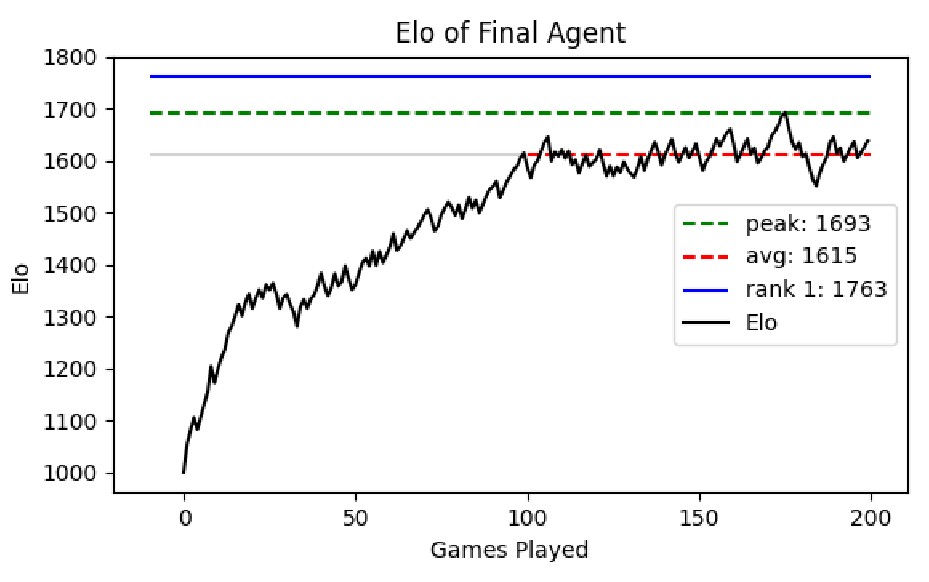
\includegraphics[width=0.7\textwidth]{figures/literature_elo.png}
    \caption{Jett Wang's Agent's ELO Rating Over 200 Games}
    \label{fig:agent_elo}
\end{figure}

The statistics provided by this research shows that the agent was able to perform at a very high competitive level, which is a great achievement for the field of RL in pokémon battling. The research also goes into detail about the observations of other experts within the field of pokémon battling \cite{wang2024winning}. Jatt Wang's research is a great example of how RL can be used to train an agent to perform at a high level in a competitive environment, where the search space for the optimal policy far larger than that of simple games such as Chess. Moreover, it proved the benefit of using PPO to train an agent to confidently perform complex pokémon battles. 

\subsection{Similar works using RL in Pokémon Red}

Despite the amount of research conducted to single objective RL in pokémon battling, there is a lack of research conducted to multi-objective RL in pokémon red. However, there is one research paper that has been conducted to train an agent to complete pokémon red using RL.

A research conducted by Flaherty, Jimenez and Abbasi applies RL algorithms A2C and DQN to play Pokémon Red from scratch called, ``Playing Pokémon Red with Reinforcement Learning''\cite{flaherty2021playing}. Compared to the other work within the field of RL using pokémon, their work focuses on comparing A2C to DQN to see if RAM observations performed better than image observations for training agents \cite{flaherty2021playing}. Despite similarities between their research and the purpose of this research, the research by Flaherty, Jimenez and Abbasi compares the performance of A2C and DQN using RAM or image observations, while this research aims to compare the performance of PPO, A2C, QRDQN and DQN using RAM and image observations with a focus on the use of multi-objective RL. This is a crutial detail to note, as the implementation of the environment by Flaherty, Jimenez and Abbasi uses different reward functions depending on if the agent was within a pokémon battle or having to navigate around the world. This means that the agent is trained to perform single objective RL by converting a multi-objective environment into a single objective environment through the use of excessive reward shaping to guide the agent to complete the game. This research paper will extend upon their research by applying and comparing more algorithms and various RL techniques to find the optimal method to complete the game.

